\documentclass[border=5pt]{standalone}
\usepackage{tikz}
\usepackage[dvipsnames]{xcolor}
\begin{document}
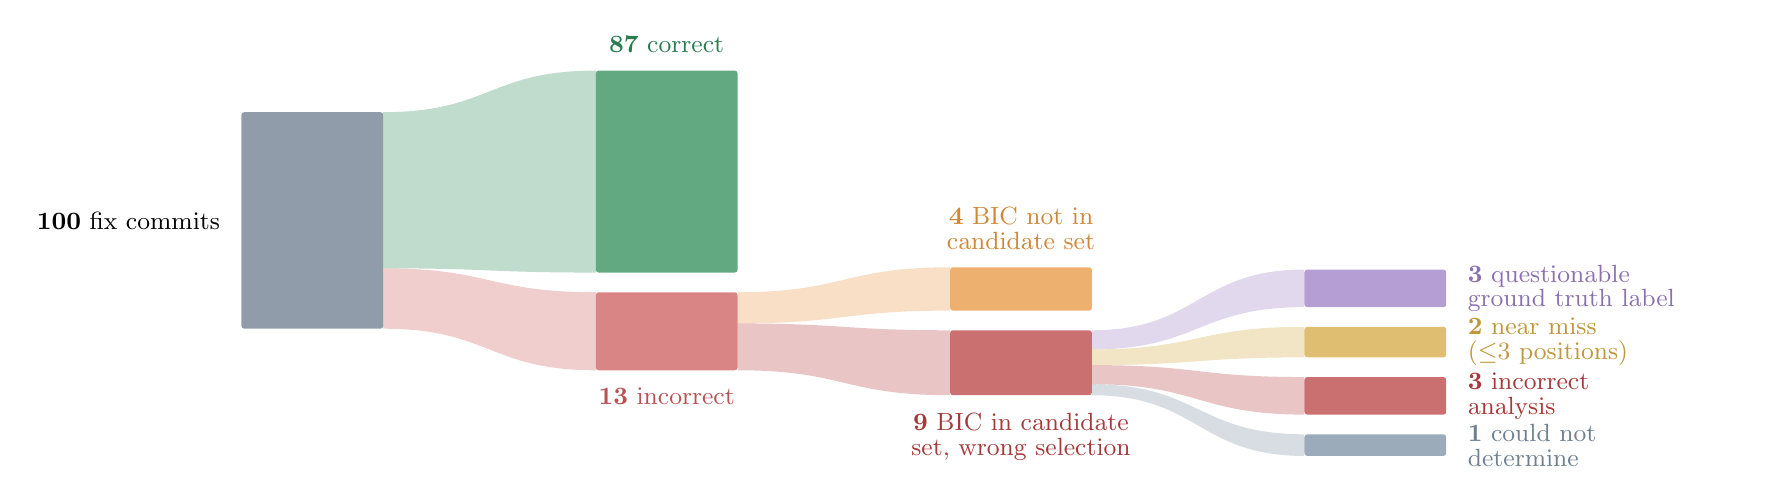
\begin{tikzpicture}[x=1cm, y=1cm]

% Color definitions
\definecolor{clCorrect}{HTML}{2E8B57}
\definecolor{clIncorrect}{HTML}{CD5C5C}
\definecolor{clNoGT}{HTML}{E8963E}
\definecolor{clQuestionable}{HTML}{9B7DC4}
\definecolor{clNearMiss}{HTML}{D4A843}
\definecolor{clWrongSel}{HTML}{B84040}
\definecolor{clCouldNotDet}{HTML}{7B8FA1}
\definecolor{clTotal}{HTML}{6B7B8D}

% Column 0: All fix commits
\fill[clTotal, opacity=0.75, rounded corners=1pt] (0.000,0.000) rectangle (1.800,2.750);

% Column 1: Correct / Incorrect
\fill[clCorrect, opacity=0.75, rounded corners=1pt] (4.500,0.713) rectangle (6.300,3.278);
\fill[clIncorrect, opacity=0.75, rounded corners=1pt] (4.500,-0.528) rectangle (6.300,0.463);

% Column 2: BIC not in candidates / BIC in candidates
\fill[clNoGT, opacity=0.75, rounded corners=1pt] (9.000,0.230) rectangle (10.800,0.780);
\fill[clWrongSel, opacity=0.75, rounded corners=1pt] (9.000,-0.845) rectangle (10.800,-0.020);

% Column 3: Detailed breakdown
\fill[clCouldNotDet, opacity=0.75, rounded corners=1pt] (13.500,-1.616) rectangle (15.300,-1.341);
\fill[clWrongSel, opacity=0.75, rounded corners=1pt] (13.500,-1.091) rectangle (15.300,-0.614);
\fill[clNearMiss, opacity=0.75, rounded corners=1pt] (13.500,-0.364) rectangle (15.300,0.024);
\fill[clQuestionable, opacity=0.75, rounded corners=1pt] (13.500,0.274) rectangle (15.300,0.751);

% Bands: Col 0 -> Col 1
\fill[clCorrect, opacity=0.30] (1.800,0.767) .. controls (3.150,0.767) and (3.150,0.713) .. (4.500,0.713) -- (4.500,3.278) .. controls (3.150,3.278) and (3.150,2.750) .. (1.800,2.750) -- cycle;
\fill[clIncorrect, opacity=0.30] (1.800,0.000) .. controls (3.150,0.000) and (3.150,-0.528) .. (4.500,-0.528) -- (4.500,0.463) .. controls (3.150,0.463) and (3.150,0.767) .. (1.800,0.767) -- cycle;

% Bands: Col 1 -> Col 2
\fill[clNoGT, opacity=0.30] (6.300,0.067) .. controls (7.650,0.067) and (7.650,0.230) .. (9.000,0.230) -- (9.000,0.780) .. controls (7.650,0.780) and (7.650,0.463) .. (6.300,0.463) -- cycle;
\fill[clWrongSel, opacity=0.30] (6.300,-0.528) .. controls (7.650,-0.528) and (7.650,-0.845) .. (9.000,-0.845) -- (9.000,-0.020) .. controls (7.650,-0.020) and (7.650,0.067) .. (6.300,0.067) -- cycle;

% Bands: Col 2 (BIC in candidates) -> Col 3
\fill[clCouldNotDet, opacity=0.30] (10.800,-0.845) .. controls (12.150,-0.845) and (12.150,-1.616) .. (13.500,-1.616) -- (13.500,-1.341) .. controls (12.150,-1.341) and (12.150,-0.705) .. (10.800,-0.705) -- cycle;
\fill[clWrongSel, opacity=0.30] (10.800,-0.705) .. controls (12.150,-0.705) and (12.150,-1.091) .. (13.500,-1.091) -- (13.500,-0.614) .. controls (12.150,-0.614) and (12.150,-0.462) .. (10.800,-0.462) -- cycle;
\fill[clNearMiss, opacity=0.30] (10.800,-0.462) .. controls (12.150,-0.462) and (12.150,-0.364) .. (13.500,-0.364) -- (13.500,0.024) .. controls (12.150,0.024) and (12.150,-0.263) .. (10.800,-0.263) -- cycle;
\fill[clQuestionable, opacity=0.30] (10.800,-0.263) .. controls (12.150,-0.263) and (12.150,0.274) .. (13.500,0.274) -- (13.500,0.751) .. controls (12.150,0.751) and (12.150,-0.020) .. (10.800,-0.020) -- cycle;

% Labels
\node[anchor=east, font=\small] at (-0.150,1.375) {\textbf{100} fix commits};
\node[anchor=south, font=\small, text=clCorrect!90!black] at (5.400,3.378) {\textbf{87} correct};
\node[anchor=north, font=\small, text=clIncorrect!90!black] at (5.400,-0.628) {\textbf{13} incorrect};
\node[anchor=south, font=\small, text=clNoGT!90!black, text width=3.5cm, align=center] at (9.900,0.880) {\textbf{4} BIC not in\\[-2pt]candidate set};
\node[anchor=north, font=\small, text=clWrongSel!90!black, text width=3.5cm, align=center] at (9.900,-0.945) {\textbf{9} BIC in candidate\\[-2pt]set, wrong selection};
\node[anchor=west, font=\small, text=clCouldNotDet!90!black, text width=3.5cm] at (15.450,-1.478) {\textbf{1} could not\\[-2pt]determine};
\node[anchor=west, font=\small, text=clWrongSel!90!black, text width=3.5cm] at (15.450,-0.853) {\textbf{3} incorrect\\[-2pt]analysis};
\node[anchor=west, font=\small, text=clNearMiss!90!black, text width=3.5cm] at (15.450,-0.170) {\textbf{2} near miss\\[-2pt]($\leq$3 positions)};
\node[anchor=west, font=\small, text=clQuestionable!90!black, text width=3.5cm] at (15.450,0.513) {\textbf{3} questionable\\[-2pt]ground truth label};

\end{tikzpicture}
\end{document}
